\documentclass[12pt, letterpaper, twoside]{article}
\usepackage{nopageno,epsfig, amsmath, amssymb}
\usepackage{physics}
\usepackage{mathtools}
\usepackage{hyperref}
\usepackage{xcolor}
\usepackage{mhchem}
\usepackage{array}
\hypersetup{
    colorlinks,
    linkcolor={blue},
    citecolor={blue},
    urlcolor={blue}
}
\usepackage{empheq}
\usepackage{wrapfig}

\usepackage[letterpaper,
            margin=0.8in]{geometry}

\newcommand{\psetnum}{5}
\newcommand{\class}{ASTR 541 - Interstellar Medium}

\newcommand{\tomtitle}{
    \noindent {\LARGE \fontfamily{cmr}\selectfont \textbf{\class}} \hfill \\[1\baselineskip]
    \noindent {\large \fontfamily{cmr}\selectfont Problem Set \psetnum \hfill \textsc{Tom Wagg}}\\[0.5\baselineskip]
    {\fontfamily{cmr}\selectfont \textit{\today}}\\[2\baselineskip]
}

\title{\class : Week \psetnum}
\author{\textbf{Tom Wagg}}

\newcommand{\question}[1]{{\noindent \it #1}}
\newcommand{\answer}[1]{
    \par\noindent\rule{\textwidth}{0.4pt}#1\vspace{0.5cm}
}
\newcommand{\todo}[1]{{\color{red}\begin{center}TODO: #1\end{center}}}

% custom function for adding units
\makeatletter
\newcommand{\unit}[1]{%
    \,\mathrm{#1}\checknextarg}
\newcommand{\checknextarg}{\@ifnextchar\bgroup{\gobblenextarg}{}}
\newcommand{\gobblenextarg}[1]{\,\mathrm{#1}\@ifnextchar\bgroup{\gobblenextarg}{}}
\makeatother

\newcommand{\avg}[1]{\left\langle #1 \right\rangle}
\newcommand{\angstrom}{\mbox{\normalfont\AA}}
\allowdisplaybreaks

\newcolumntype{C}{>{$}c<{$}}

\begin{document}

\tomtitle{}

\noindent For reference, if you'd ever like to see the code that I've used to get my answers to these, \href{https://github.com/TomWagg/uw-grad-classes/tree/main/541_ism}{here's a link to my GitHub repo}! (\#astropy.units for life)\\

\question{\textbf{1. SII Transitions}}


\begin{center}
    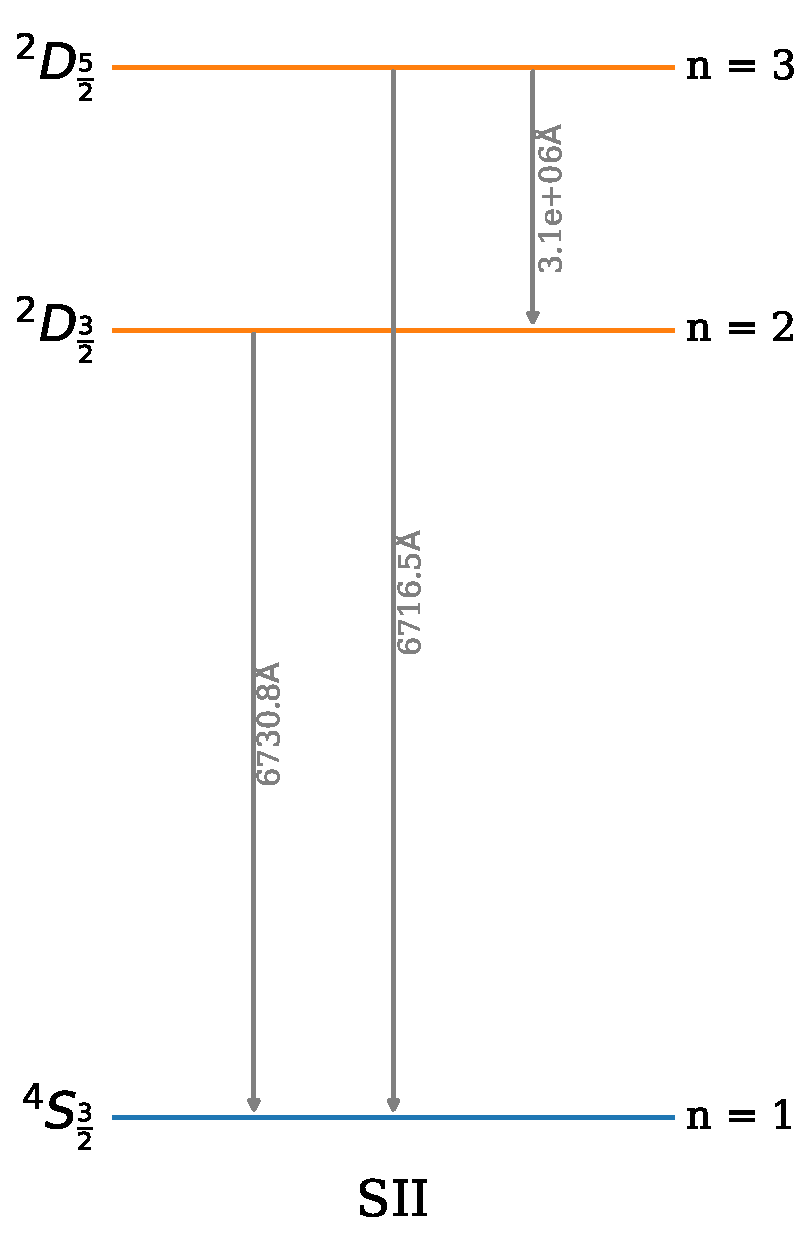
\includegraphics[width=0.5\textwidth]{energy_levels.pdf}
\end{center}

\question{1a. Electronic Configuration}
\answer{
    I used my Python program (and the Aufbau Principle) to find that the electronic configuration of SII is
    \begin{equation}
        \boxed{ \mathrm{SII} = 1s^2 2s^2 2p^6 3s^2 \mathbf{3p^3} }
    \end{equation}
    where the last subshell is only half-filled and so this is where we get our terms.
}

\question{1b. Spectroscopic Terms}
\answer{
    Again I put my feet up and let Python do the heavy lifting to find (and sort!) the spectroscopic terms as
    \begin{equation}
        \boxed{ \mathrm{SII} = {}^4\mathrm{S}_{3/2}, {}^2\mathrm{D}_{3/2,\, 5/2}, {}^2\mathrm{P}_{1/2,\, 3/2}}
    \end{equation}
    and additionally plug those into a plotting function to get the diagram above.
}

\question{1c. Cooling Rate}
\answer{
    As noted in the question, the cooling rate per SII ion is calculated as the sum of line intensities. We can therefore write the cooling rate per ion as a product of sums.
    \begin{equation}
        I = \sum_{i = 2}^{3} \sum_{j = 1}^{i - 1} \frac{n_i}{n_{\rm SII}} A_{ij} \Delta E_{ij}
    \end{equation}
    where $n_i / n_{\rm SII}$ is the fraction of ions that are in state $i$ (table 2 from the question), $A_{ij}$ is the Einstein coefficient for the transition from $i$ to $j$ (table 1 from the question) and $\Delta E_{ij}$ is the difference in energy between states $i$ and $j$ (table 1 from the question). Then we plug, we chug, we put it all in a table.
    \begin{center}
        \boxed{\begin{tabular}{C|C}
            n_e [\unit{cm^{-3}}] & I [\unit{erg}{s^{-1}}{ion^{-1}}]\\
            \hline
            10   & 5.15 \times 10^{-19} \\
            10^3 & 4.36 \times 10^{-17} \\
            10^5 & 3.17 \times 10^{-16}
        \end{tabular}}
    \end{center}
}

\question{1d. Excitation Temperature}
\answer{
    The excitation temperature for a transition from $u$ to $l$ can be written as
    \begin{equation}
        e^{-E_{ul} / k_B T_{\rm ex}} = \frac{n_u}{n_l} \frac{g_l}{g_u}
    \end{equation}
    Or if we rearrange it
    \begin{equation}
        T_{\rm ex} = - \frac{E_{ul}}{k_B} \qty(\ln \frac{n_u}{n_l} \frac{g_l}{g_u})^{-1}
    \end{equation}
    The transition from ${}^2\mathrm{D}_{3/2} \to {}^4\mathrm{S}_{3/2}$ corresponds to a transition from $n=2$ to $n=1$ in our labelling scheme. The degeneracies of these two states are identical so we can cancel the $g$ factors. It is then simply a matter of plugging in the $\Delta E$ and $n$ values from the tables in the question to get values for the temperature.
    \begin{center}
        \boxed{\begin{tabular}{C|C}
            n_e [\unit{cm^{-3}}] & T_{\rm ex} [\unit{K}]\\
            \hline
            10   & 2.3 \times 10^{3} \\
            10^3 & 4.6 \times 10^{3} \\
            10^5 & 9.6 \times 10^{3}
        \end{tabular}}
    \end{center}
}

\question{1e. Trends}
\answer{
    We can summarise the trends in a table by looking at the ratio of the cooling rates and temperatures to the initial electron density values. We see that the cooling rates and excitation temperatures both increase with increasing electron densities.
    \begin{center}
        \begin{tabular}{C|C|C}
            n_e [\unit{cm^{-3}}] & I / I(n_e = 10 \unit{cm^{-3}}) & T_{\rm ex} / T_{\rm ex}(n_e = 10 \unit{cm^{-3}})\\
            \hline
            10   & 1 & 1 \\
            10^3 & 85 & 2.01 \\
            10^5 & 620 & 4.22
        \end{tabular}
    \end{center}
    The cooling rate increases since a higher electron density results in more collisions and more ions in excited states (collisions are exciting!) - this results in more transitions and more emissions and thus more cooling. The excitation temperature increases since it corresponds to the internal energy of the ions and so more collisions and more excited ions implies a higher excitation temperature.

    If we were to increase the density even higher the excitation temperature would eventually level off at it reaches equilibrium with the kinetic temperature of the gas (${\sim}10000\unit{K}$).
}

\question{1f. Diagnostics}
\answer{
    Given that the change in energy between the $n=2$ and $n=3$ states is small, the emission line intensity ratio would be a useful diagnostic for \textbf{density}.
}

\question{1g. Low Density Ratios}
\answer{
    The ratio of the intensities in a low density regime is given by
    \begin{equation}
        \frac{I_{31}}{I_{21}}_{n \ll n_{\rm crit}} = \frac{\Omega_{31}}{\Omega_{21}}
    \end{equation}
    I \emph{could} look these values up and plug them in, \emph{or} I could be lazy and just take a look at Figure 18.4 from Draine and read off the ratio. I will leave it as an exercise to the reader to guess which method I used.
    \begin{equation}
        \boxed{ \frac{I_{31}}{I_{21}}_{n \ll n_{\rm crit}} \approx 1.44 }
    \end{equation}
}

\question{1h. High Density Ratios}
\answer{
    The ratio of the intensities in a high density regime is given by
    \begin{equation}
        \frac{I_{31}}{I_{21}}_{n \gg n_{\rm crit}} = \frac{g_3}{g_2} \frac{A_{31}}{A_{21}}
    \end{equation}
    We know all of these values (recalling $g = 2 J + 1$), and so plugging them in we find
    \begin{equation}
        \boxed{ \frac{I_{31}}{I_{21}}_{n \gg n_{\rm crit}} \approx 0.44 }
    \end{equation}
}

\end{document}

 